% %% %%%%%%%%%%%%%%%%%%%%%%%%%%%%%%%%%%%%%%%%%%%%%%%%%%%%%%%%%%
% step-1.tex
%
% Author:  Mauricio Matamoros
% License: MIT
%
% %% %%%%%%%%%%%%%%%%%%%%%%%%%%%%%%%%%%%%%%%%%%%%%%%%%%%%%%%%%%

%!TEX root = ../practica.tex
%!TEX root = ../references.bib

% CHKTEX-FILE 1
% CHKTEX-FILE 13
% CHKTEX-FILE 46

\subsection{Paso 1: Alambrado}%
\label{sec:step1}

El proceso de alambrado de esta práctica considera dos circuitos.
El primer circuito, mostrado en la \Cref{fig:lm35-arduino}, permite obtener valores discretos del sensor de temperatura LM35.
El segundo circuito (\Cref{fig:circuit-full}) consiste en la interfaz de conexión vía \IIC entre el microcontrolador que lee el LM35 y la Raspberry Pi que genera los reportes y grafica los resultados.

\begin{wrapfigure}[14]{r}{0.33\columnwidth}
	\vspace{-5mm}
	\centering
	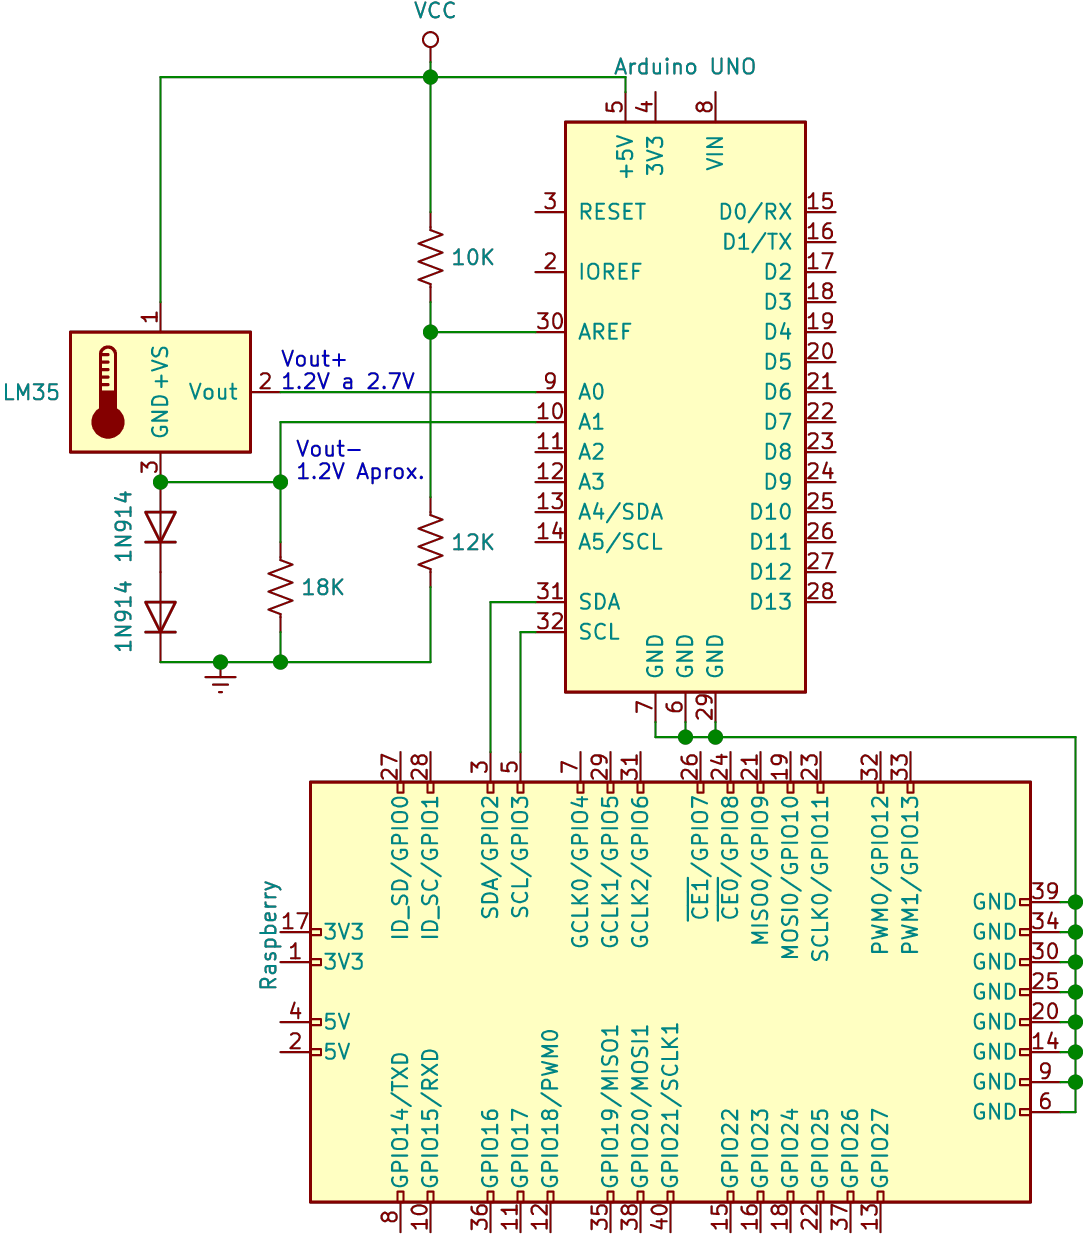
\includegraphics[width=0.5\columnwidth,height=7cm,keepaspectratio]{img/lm35-arduino-pi.png}
	\caption{Circuito completo}
	\label{fig:circuit-full} % CHKTEX 24
\end{wrapfigure}

Alambre primero el subcircuito formado por los dos diodos, el integrado LM35 y la resistencia de 18k$\Omega$.
Paso seguido, alimente el subcircuito con 5V y mida la diferencia de potencial existente entre V\textsubscript{OUT-} y \GND{}.
Utilice el valor medido en la fórmula $V_{AREF} = 1.5V + V_{OUT-}$ para calcular los valores de las resistencias que se conectarán al pin AREF del Arduino.

% \paragraph*{IMPORTANTE:}
\medskip
\begin{importantbox}{\large Importante}
	\begin{center}
		Asegúrese de que $V_{AREF} \leq V_{OUT-}\Big|_{Temp=150^{o}C}$ para evitar quemar el Arduino.
	\end{center}
\end{importantbox}
\medskip

Continúe el alambrado del circuito.
Es conveniente colocar un capacitor de 0.1$\mu$F entre \VCC y \GND para rectificar el voltaje de entrada eliminar cualquier oscilación parásita que pudiere afectar el funcionamiento del LM35.
La presencia de este componente es opcional pero altamente recomendada.

\medskip
Tras alambrar el primer circuito realice el experimento prueba indicado en la \Cref{sec:step2}.
\medskip

\begin{wrapfigure}[11]{r}{5cm}
	\vspace{-5mm}
	\centering
	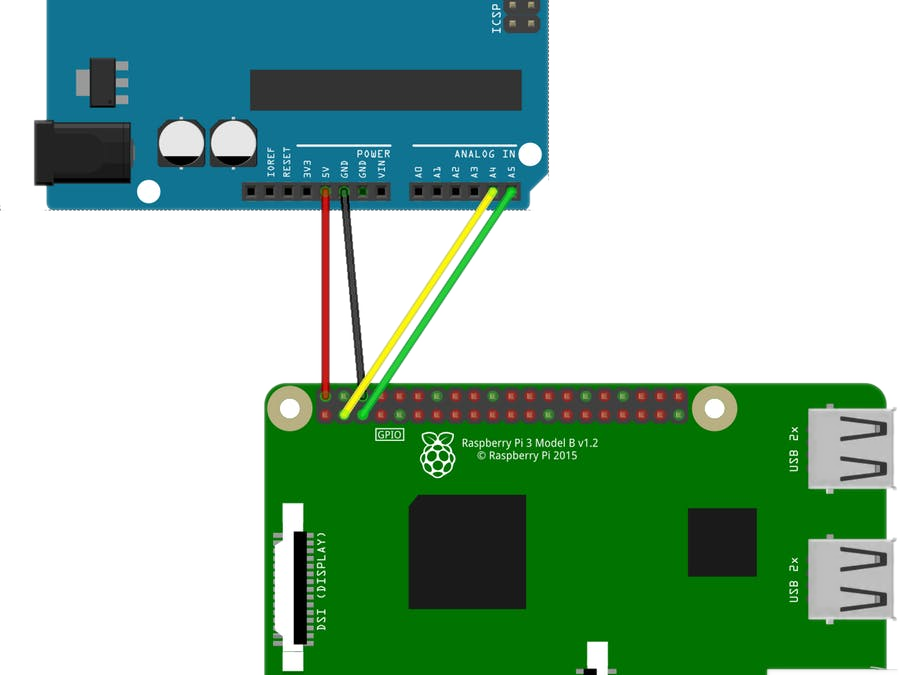
\includegraphics[width=\linewidth]{img/pi-arduino-i2c.png}
	\caption[Conexión de una Raspberry Pi con un Arduino UNO via \IIC]{Conexión mediante \IIC de una Raspberry Pi con un Arduino UNO\footnotemark}%
	\label{fig:pi-arduino-i2c} % CHKTEX 24
\end{wrapfigure}
\footnotetext{Imagen obtenida de \url{https://create.arduino.cc/projecthub/aardweeno/59817b}}

A continuación conecte el bus \IIC entre la Raspberry Pi y el Arduino como ilustran la \Cref{tbl:pi-arduino-i2c} y la \Cref{fig:pi-arduino-i2c}.
Hay tutoriales que sugieren utilizar un convertidor de niveles de voltaje cuando se conecta una Raspberry Pi a un arduino mediante \IIC, especialmente cuando la Raspberry Pi opera a 3.3V.
Esto \textbf{NO} es necesario si la Raspberry Pi está configurada como dispositivo maestro o \emph{master} y el Arduino como dispositivo esclavo o \emph{slave}.


\begin{table}
	\centering
	\caption{Conexiones \IIC entre Raspberry Pi y un Arduino}
	\label{tbl:pi-arduino-i2c} % CHKTEX 24
	\begin{tabularx}{0.8\linewidth}{cc rcl c c}
	\toprule
	\multicolumn{2}{c}{   Pin   } & \multicolumn{3}{c}{\multirow{2}{*}{Conexión}}  &     Pin     &     Pin     \\
	\multicolumn{2}{c}{Raspberry} & \multicolumn{3}{c}{}                           & Arduino UNO & Arduino Mega \\
	\midrule
	       3 & (GPIO2)            & Raspberry Pi SDA & $\rightarrow$ & Arduino SDA & A4          & SDA (PIN 20) \\
	       5 & (GPIO3)            & Raspberry Pi SCL & $\rightarrow$ & Arduino SCL & A5          & SCL (PIN 21) \\
	       6 & (\GND)             & Raspberry Pi GND & $\rightarrow$ & Arduino GND & \GND        & \GND         \\
	\bottomrule
	\end{tabularx}
\end{table}


Esto es posible debido a que el Arduino no tiene resistencias de acoplamiento a positivo o \emph{pull-up} integradas, mientras que los pines \IIC de la Raspberry Pi están conectados internamente a la línea de 3.3V mediante resistencias de 1.8k$\Omega$.
Por este motivo, tendrán que quitarse las resistencias de \emph{pull-up} a cualquier otro dispositivo esclavo que se conecte al bus \IIC de la Raspberry Pi.\footnote{Para más información sobre el papel de las resistencias de acoplamiento a positivo o \emph{pull-up} en un bus \IIC se puede consultar \url{http://dsscircuits.com/articles/effects-of-varying-i2c-pull-up-resistors} }
